\documentclass[a4paper,12pt,openany]{book}

\usepackage[utf8]{inputenc}
\usepackage{graphicx}
\usepackage[pdftex,colorlinks,citecolor=black,filecolor=black,linkcolor=black,urlcolor=black,pagebackref]{hyperref}

\oddsidemargin 1.4cm
\evensidemargin 0.35cm
\textwidth 14cm
\topmargin 0.26cm
\headheight 0.6cm
\headsep 1.5cm
\textheight 20cm

\newcommand{\CcImageCc}[1]{%
	
\includegraphics[scale=#1]{cc.eps}%
}
\newcommand{\CcImageBy}[1]{%
	\includegraphics[scale=#1]{by.eps}%
}
\newcommand{\CcImageSa}[1]{%
	
\includegraphics[scale=#1]{sa.eps}%
}

\begin{document}

\thispagestyle{empty}

\vspace*{5cm}
{\small \noindent
To delo je ponujeno pod licenco \textit{Creative Commons Attribution-ShareAlike International 4.0 (CC BY-SA 4.0)}.
To pomeni, da se tako besedilo, slike, grafi in druge sestavine dela kot tudi rezultati diplomskega dela lahko prosto distribuirajo,
reproducirajo, uporabljajo, priobčujejo javnosti in predelujejo, pod pogojem, da se jasno in vidno navede avtorja in naslov tega
dela in da se v primeru spremembe, preoblikovanja ali uporabe tega dela v svojem delu, lahko distribuira predelava le pod
licenco, ki je enaka tej.
Podrobnosti licence so dostopne na spletni strani \href{http://creativecommons.org/licenses/by-sa/4.0/}{creativecommons.org}.

\begin{center}% 0.66 / 0.89 = 0.741573033707865
\CcImageCc{0.4}\hspace*{1ex}\CcImageBy{0.4}\hspace*{1ex}\CcImageSa{0.4}%
\end{center}
}

\vspace*{1.5cm}
{\small \noindent
Izvorna koda diplomskega dela, njeni rezultati in v ta namen razvita programska oprema je ponujena pod licenco MIT. To pomeni, da se lahko prosto distribuira in/ali predeluje pod njenimi pogoji.
Podrobnosti licence so dostopne na spletni strani \url{http://opensource.org/licenses/MIT}.
Izvorna koda je dostopna na naslovu \url{https://github.com/sstanovnik/ParallelTimetables}.
}

\begin{center} 
\ \\ \vfill
{\em
Besedilo je oblikovano z urejevalnikom besedil \LaTeX.}
\end{center}

\end{document}
